\section{Governo Digital}

O advento da internet surgiu e reconfigurou o meio de comunicação para a população e, com o advento e evolução da tecnologia 
e expansão da internet surge a expressão \textit{Governo Digital}. Esta expressão se refere ao uso de tecnologias digitais como uma 
estratégia de modernização do Governo, que adota a tecnologia da informação e comunicação (TIC) para prover 
serviços e maximizar a eficiência de atividades governamentais~\cite{fang2002government}. 

O termo \textit{e-Governo} surgiu no final da década de 1990 e cresceu consideravelmente com 
diversas definições, como: governo mais eficiente, melhores serviços para o cidadão e um melhor processo 
democrático. Em sequência, nos últimos anos, o termo \textit{e-Governo} deu origem a várias conferências de cunho científico, aumentando seu 
conteúdo e posição no que se refere a outros campos de pesquisa e disciplinas~\cite{gronlund2005introducing}.

A OECD (Organisation for Economic Co-operation and Development) usa a expressão \textit {Governo Eletrônico} como o uso de 
Tecnologias de Informação e Comunicação pelo governo, que se refere a uma ferramenta que busca melhorar as atividades do governo, 
especialmente, com do uso da Internet. A expressão \textit{Governo Digital}, por outro lado, refere-se ao uso de tecnologias 
digitais que buscam adicionar valor público como parte complementar às estratégias de modernização de um governo.

A integração de novas tecnologias no cotidiano faz com que as expectativas dos cidadãos sobre suas relações com os governos mudem~\cite{oecd}, visto que as opiniões e necessidades podem passar a ser consideradas de forma mais eficaz, trazendo a possibilidade 
de realizar processos governamentais com maior facilitade e agilidade. Esta consolidação das expectativas criadas sobre o governo exige que novas abordagens de governança pública possam trazer a digitização de serviços,
considerando-se que, através da desburocratização de alguns serviços e processos, os cidadãos e empresas podem ser integrados ao meio digital.

Embora as medidas de modernização do setor público tenham começado a ser adotadas na década de 70, a dedicação, de fato, apareceu apenas em decorrência da crise fiscal dos anos 80, quando a intervenção estatal se popularizou como reforma da gestão pública que, aliada às TICs, disponibilizou serviços públicos eletrônicos à população no início da década de 2000~\cite{przeybilovicz2015desenvolvimento}.

O conceito de E-governo envolve um aglomerado de responsabilidades que impactam em todos os níveis sociais. De acordo com \cite{fang2002government}, o conceito de E-governo possui três grandes focos: 

\begin{itemize}
    \item \textbf{E-Government}: Referente as atividades internas do governo, sejam administrativas, organizacionais ou de comunicação. 
    \item \textbf{E-Commerce}: Responsável pela interface entre o governo e o mercado.
    \item \textbf{E-Citizens}: Suporte para interface entre governo e cidadão, possibilitando a disponibilização de serviços de maneira prática e eficiente.
\end{itemize}

A Figura \ref{img:triangulo} apresenta o modelo de relacionamento entre E-Government, E-Commerce e E-Citizens.

\begin{figure}[!htb]
\centering
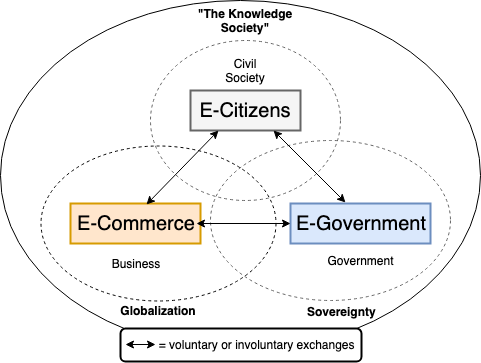
\includegraphics[width=.8\textwidth]{figuras/relacao_triangular_e-gov.png}
\caption{Triangle Relationship Model: E-Government, Business and Citizens. Adaptado de \cite{fang2002government}.}
\label{img:triangulo}
\end{figure}

Neste sentido, o conceito de Governo Digital envolve diversos âmbitos, evidenciando a grandeza e importância de um processo de transformação digital no governo.


\section{Transformação Digital no Brasil}

No Brasil, em 2016, somente 54\% dos domicílios brasileiros possuíam acesso à internet, o que representa 6,7 milhões de residências e um total de 107,9 milhões de usuários de Internet~\cite{CGI}. Neste mesmo ano, ocorreu o lançamento da \textit{Estratégia de Governança Digital da Administração Pública Federal} (EGD), com o objetivo de definir estratégias, metas e indicadores da Política de Governança Digital. A partir da EGD, a prestação de serviços
públicos poderia ser simplificada e agilizada proporcionando uma melhoria no ambiente de negócios e eficiência da gestão pública.

Ainda em 2016, o Decreto número 8.638 foi publicado pela Casa Civil da Presidência da República \cite{BRASIL2016c}, instituindo a Política de Governança Digital, no âmbito dos órgãos e das entidades da administração pública federal direta, autárquica e fundacional. 

% No Decreto número 8.638 \cite{BRASIL2016c}, existem dois artigos a serem destacados por seus princípios e objetivos, estes estão 
% listados na tabela a seguir:

Para estimular a transformação dos serviços públicos em serviços digitais, de modo que estes ocorram por meio eletrônico, o governo
brasileiro publicou decretos relevantes entre 2014 e 2016, como citado ao longo desta seção. Os decretos definiram a Política de Governança
Digital e a Plataforma de Cidadania Digital, no âmbito da Administração Pública Federal (APF), ambos de responsabilidade do então 
Ministério do Planejamento, Desenvolvimento e Gestão (MP) anos \cite{BRASIL, BRASIL2016}. 

A Plataforma de Cidadania Digital configura um conjunto de metodologias e soluções que buscam ampliar e simplificar o acesso dos cidadãos aos serviços digitais e, também, para apoiar os órgãos públicos na aceleração da transformação digital de serviços.  

Simultaneamente às ações da Plataforma de Cidadania Digital, o Departamento lançou um canal para oferecer informações no
formato de um portal de serviços do Governo Federal\footnote{https://www.servicos.gov.br/}. A iniciativa surgiu para permitir o arquivamento de solicitações eletrônicas e monitorar os serviços públicos pelos usuários. Juntamente com o portal, foi lançado um programa de automação de serviços públicos, para a tentativa de orientar e apoiar órgãos públicos a identificar, priorizar, digitalizar e implementar serviços 
com mais qualidade e transparência para os cidadãos.

Um dos objetivos do governo brasileiro com a transformação digital é ampliar os serviços públicos nos canais digitais. 
Atualmente, o governo oferece aproximadamente 1.700 serviços, mas apenas 41\% são totalmente digitais. Vale ressaltar que o processo de transformação brasileiro envolve os três principais focos apresentados na Figura \ref{img:triangulo}: \textit{E-Government}, \textit{E-Commerce} e \textit{E-Citizens}.

Tendo em vista os decretos publicados, o Departamento \textbf{INOVA} do antigo MP, se responsabilizou pela construção de um programa de Governo Digital, denominado \textit{Kit de Transformação}. O objetivo é, de modo geral, transformar os serviços públicos a partir da utilização de um kit, ao invés da adoção de uma metodologia, por exemplo, objetivando facilitar a adoção e orientação aos diversos órgãos da APF.

O \textit{Kit de Transformação} é composto por seis estágios de aplicações independentes, como demonstrado na Figura \ref{fig:EtapasTransform}.

        \begin{figure}[h]
          \centering
          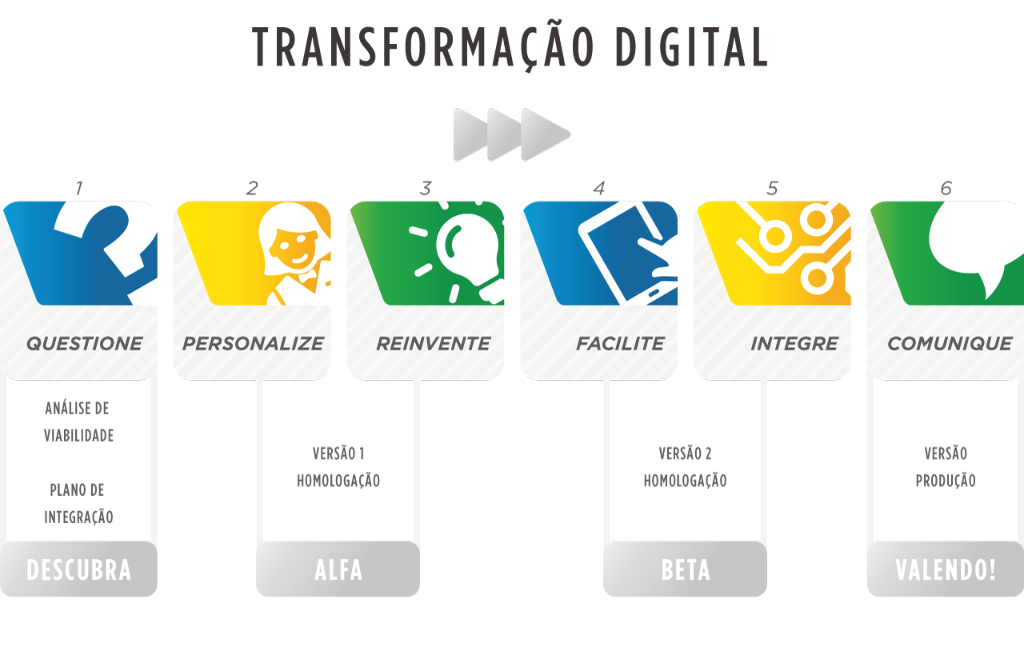
\includegraphics[width=15cm]{figuras/secao-referencial/EtapasTransform.png}
          \caption{Fases do Kit de Transformação (Fonte: \cite{BRASIL2017})} 
          \label{fig:EtapasTransform}
        \end{figure}
        
        
A seguir é apresentado cada um dos estágios destacados na Figura \ref{fig:EtapasTransform}:

\begin{itemize}
\item \textbf{Questione}

Esta fase foi delineada para que o órgão fosse capaz de identificar e priorizar seus principais serviços, além de realizar um diagnóstico que anteceda a transformação, de modo que uma avaliação posterior resulte nos anseios dos usuários. A metodologia desta fase busca, especificamente, a identificação de serviços, avaliação da maturidade da gestão em serviços, levantamento de custos dos usuários do serviço, priorização da transformação de serviços e, por fim, o diagnóstico e avaliação dos serviços.

\item \textbf{Personalize}
Nesta fase é utilizada a visão do usuário como um propósito para que se atinja serviços personalizados, sendo assim, o ministério busca identificar as necessidades do usuário afundo para que se mapeie as impressões mais relevantes sobre os problemas levantados. A partir do levantamento das necessidades mais relevantes dos usuários, pode-se conseguir dados sobre o acesso, uso, satisfação e expectativas sobre o serviço prestado, além da análise de qualidade do serviço em questão.


\item \textbf{Reinvente}


É importante que a transformação seja analisada, sintetizada, prototipada e testada, por isso, esta fase realiza a definição do Serviço Mínimo Viável (SMV). Partindo desta definição torna-se possível escolher alternativas de solução e possibilidades de se encontrar um melhor trajeto para a iniciação da transformação de serviços. É fundamental nesta fase que se crie novas soluções para aprimorar e estimular o processo de transformação deste contexto.


\item \textbf{Facilite}


A ideia da fase Facilite é oferecer um guia de simplificação de serviços ao participante. É a partir desta fase que se configuram ferramenta de agendamentos, ferramenta de automação de serviços públicos, solução de peticionamento eletrônico do SEI (Sistema Eletrônico de Informações) e solução de atendimento virtual.



\item \textbf{Integre}


Ao solicitar um serviço, o cidadão precisa disponibilizar tempo e custo logístico para obter a apresentar determinados documentos que são requeridos. Sendo assim, o objetivo desta fase é integrar suas bases de dados às plataformas criadas de modo que, o acesso dos cidadãos aos serviços sejam simplificados, com dados unificados. Com a integração das informações dos usuários pode-se eliminar a necessidade de que se apresente dados já cadastrados pelo cidadão, ou seja, as bases do governo que já capturaram determinadas informações, passam a reutilizá-las em diversas situações, minimizando o esforço por parte do cidadão.


\item \textbf{Comunique}


Para que se planeje e comunique aos cidadãos as mudanças realizadas, é necessário que o órgão defina e avalie ações de comunicação. Para tanto, a fase Comunique necessita da transformação do serviço pronta para ser implantada, com seus respectivos canais de atendimento para a transformação do serviços. 

\end{itemize}

Por meio das ferramentas da fase \textit{Questione}, o órgão parceiro poderá avaliar em que medida as ferramentas das demais fases serão úteis para melhorar seus serviços. Com isso, o órgão parceiro terá parâmetros para decidir se utilizará o conjunto completo do Programa ou se adotará uma ``\textit{estratégia de prateleira}'', selecionando aleatoriamente as ferramentas de que necessita.

Para a fase Facilite, o Ministério contrata, através de um concurso de licitações, uma empresa que fornece uma ferramenta de digitalização de serviços baseada no conceito de \textit{meta-design}~\cite{fogli2012meta}. Após a digitalização, os serviços devem ser validados e entregues a população. 

O ITRAC, da UnB, em seu projeto de parceria com o então Ministério do Planejamento, contribuiu para o programa de automatização no quesito da garantia da qualidade dos serviços transformados. A figura \ref{fig:transformacao} apresenta a posição do laboratório ITRAC no processo de transformação digital dos serviços públicos brasileiros. Neste processo destacam-se, ainda, (1) a empresa \textbf{LECOM}, empresa terceirizada contratada para acelerar o processo de transformação digital dos serviços públicos, (2) o órgão parceiro (realizando o papel de ``cliente'' no processo de transformação), e (3) o Ministério do Planejamento, Desenvolvimento e Gestão.

A figura abaixo apresenta, de forma prática, como o conjunto de ferramentas e métodos distribuídos nos seis estágios independentes do kit de transformação se relacionam com o processo de validação definido pelo ITRAC.


        \begin{figure}[h]
          \centering
          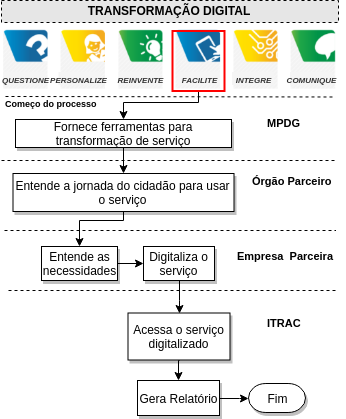
\includegraphics[width=10cm]{figuras/secao-referencial/ProcessodeContextualizacao.png}
          \caption{Processo de Transformação digital (Fonte: Adaptado de \cite{itkonen2015test})} 
          \label{fig:transformacao}
        
        \end{figure}
